Gegeben ist der Graph der Funktion $y=\frac12x^2$ (siehe
Abbildung~\ref{40000066:figure}).
\begin{teilaufgaben}
\item
Bestimmen Sie die Normalenform einer Geraden durch die beiden
Parabelpunkte mit den $x$-Koordinaten $x_0$ und $x_0+h$.
\item
Finden Sie einen Normalenvektor der eben gefundenen Geraden.
\item
Finden Sie den Grenzwert des Normalenvektors für $h\to 0$.
Dies ist der Vektor $\vec n$ in Abbildung~\ref{40000066:figure}
und die zugehörige Gerade ist die Tangente an die Kurve.
\item
Spiegeln Sie die zur $y$-Achse parallele Gerade durch $x_0$ an der in
c) gefundene Geraden.
\item
Finden Sie den Schnittpunkt der gespiegelten Geraden mit der $y$-Achse.
\end{teilaufgaben}

\begin{hinweis}
In dieser Aufgabe müssen Sie wiederholt Richtungsvektoren bestimmen und damit
weiterrechnen.
Beachten Sie und nutzen Sie aus, dass es dabei nicht auf die Länge dieser
Richtungsvektoren ankommt.
Sie können einen Richtungsvektor durch eine beliebige Zahl teilen oder
mit einer Zahl multiplizieren, so dass Sie eine möglichst handliche
Form für den Vektor erhalten.
\end{hinweis}

\begin{figure}[h]
\centering
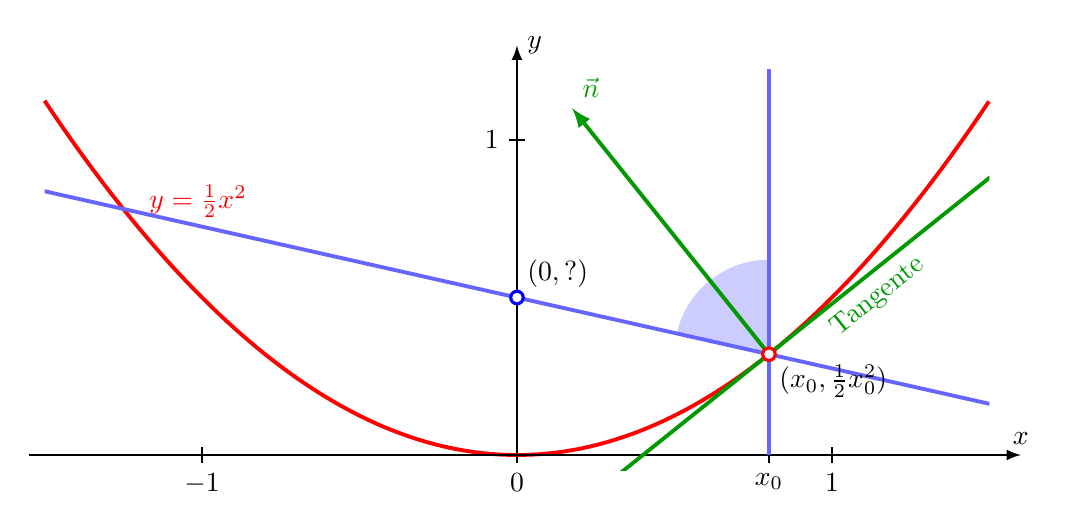
\begin{tikzpicture}[>=latex,thick,scale=4]
\definecolor{darkgreen}{rgb}{0,0.6,0}

% Parabel
\draw[color=red,line width=1.4pt]
	plot[domain=-1.5:1.5,samples=100] ({\x},{0.5*\x*\x});
\node[color=red] at (-1.2,{0.5*1.2*1.2}) [above right] {$y=\frac12x^2$};

% Koordinatenachsen
\draw[->] (-1.55,0)--(1.6,0) coordinate[label={$x$}];
\draw[->] (0,-0.025)--(0,1.3) coordinate[label={right:$y$}];

\draw (1,-0.025)--(1,0.025);
\draw (-1,-0.025)--(-1,0.025);
\node at (1,-0.025) [below] {$1$};
\node at (-1,-0.025) [below] {$-1$};
\node at (0,-0.025) [below] {$0$};
\draw (-0.025,1)--(0.025,1);
\node at (-0.025,1) [left] {$1$};

\def\xzero{0.8}
%\def\xzero{1}

\draw (\xzero,-0.025)--(\xzero,0.025);
\node at (\xzero,-0.025) [below] {$x_0$};

\pgfmathparse{0.5*(\xzero*\xzero-1)/\xzero}
\xdef\m{\pgfmathresult}

\xdef\M{\xzero}
\pgfmathparse{atan(\M)}
\xdef\a{\pgfmathresult}

\fill[color=blue!20]
	({\xzero},{0.5*\xzero*\xzero})
	--
	({\xzero},{0.5*\xzero*\xzero+0.3}) arc (90:{90+2*\a}:0.3)
	--
	cycle;
	

\pgfmathparse{sqrt(\xzero*\xzero+1)}
\xdef\l{\pgfmathresult}

\begin{scope}
\clip (-1.5,-0.05) rectangle (1.5,{0.5*1.5*1.5+0.1});
\draw[color=blue!60,line width=1.4pt] 
	(\xzero,0)--(\xzero,2);
\draw[color=blue!60,line width=1.4pt]
	(-2,{0.5-2*\m})
	--
	(2,{0.5+2*\m});

\node at (\xzero,{0.5*\xzero*\xzero}) [below right] {$(x_0,\frac12x_0^2)$};

\draw[line width=1.4pt,color=darkgreen] 
	(0,{0.5*\xzero*\xzero-\M*\xzero})
	--
	(2,{0.5*\xzero*\xzero+\M*(2-\xzero)});

\node[color=darkgreen] at ({\xzero+0.3},{0.5*\xzero*\xzero+0.3*\M})
	[below,rotate=\a] {Tangente};

\end{scope}

\draw[->,color=darkgreen,line width=1.4pt]
	({\xzero},{0.5*\xzero*\xzero})
	--
	({\xzero-\xzero/\l},{0.5*\xzero*\xzero+1/\l});
\node[color=darkgreen] at ({\xzero-\xzero/\l},{0.5*\xzero*\xzero+1/\l})
	[above right] {$\vec{n}$};


\fill[color=red]  (\xzero,{0.5*\xzero*\xzero})  circle[radius=0.025];
\fill[color=white]  (\xzero,{0.5*\xzero*\xzero})  circle[radius=0.015];

\fill[color=blue]  (0,0.5)  circle[radius=0.025];
\fill[color=white]  (0,0.5)  circle[radius=0.015];
\node at (0,0.5) [above right] {$(0,?)$};

\end{tikzpicture}
\caption{Parabel zu Aufgabe~\ref{40000066}
\label{40000066:figure}}
\end{figure}

\thema{Normalenvektor}
\thema{Normalenform}
\thema{Schnittpunkt}

\begin{loesung}
\begin{teilaufgaben}
\item
Die gesuchte Normalenform
${\color{red}a}x+{\color{red}b}y+{\color{red}c}=0$
der Geraden durch die Punkte
$(x_0,\frac12x_0^2)$ und $(x_0+h, \frac12x_0^2+x_0h+\frac12h^2)$
muss die Gleichungen
\[
\begin{linsys}{3}
{\color{red}a}\cdot x_0    &+&  {\color{red}b}\cdot \frac12x^2               &+& {\color{red}c} &=& 0\\
{\color{red}a}\cdot(x_0+h) &+&  {\color{red}b}\cdot \frac12(x_0^2+2x_0h+h^2) &+& {\color{red}c} &=& 0\\
\end{linsys}
\]
erfüllen.
Wir verwendenden den Gauss-Algorithmus, aber bevor wir mit dem
Gauss-Algorithmus beginnen, subtrahieren wir die erste Zeile von
der zweiten und teilen durch $h$.
\[
\begin{linsys}{3}
{\color{red}a}\cdot x_0 &+& {\color{red}b}\cdot \frac12x^2      &+& {\color{red}c} &=& 0\\
{\color{red}a}          &+& {\color{red}b}\cdot \frac12(2x_0+h) & &   &=& 0\\
\end{linsys}
\]
Dadurch wird das Gleichungssystem etwas einfacher, nämlich
\begin{align*}
\begin{tabular}{|>{$}c<{$} >{$}c<{$} >{$}c<{$}| >{$}c<{$}|}
\hline
% a  &    b         &c &   \\
{\color{red}a}&{\color{red}b}&{\color{red}c}&\\
\hline
x_0 &\frac12x_0^2  &1 & 0 \\
1 &\frac12(2x_0+h) &0 & 0 \\
\hline
\end{tabular}
&
\rightarrow
\begin{tabular}{|>{$}c<{$} >{$}c<{$} >{$}c<{$}| >{$}c<{$}|}
\hline
%a &    b                      &      c        &   \\
{\color{red}a}&{\color{red}b}&{\color{red}c}&\\
\hline
1 &\frac12x_0                 &\frac1x_0      & 0 \\
0 &\frac12(2x_0+h)-\frac12x_0 &-\frac{1}{x_0} & 0 \\
\hline
\end{tabular}
=
\begin{tabular}{|>{$}c<{$} >{$}c<{$} >{$}c<{$}| >{$}c<{$}|}
\hline
%a &    b            &      c        &   \\
{\color{red}a}&{\color{red}b}&{\color{red}c}&\\
\hline
1 &\frac12x_0       &\frac1x_0      & 0 \\
0 &\frac12(x_0+h)  &-\frac{1}{x_0} & 0 \\
\hline
\end{tabular}
\\
\rightarrow
\begin{tabular}{|>{$}c<{$} >{$}c<{$} >{$}c<{$}| >{$}c<{$}|}
\hline
% a  &    b   &      c &   \\
{\color{red}a}&{\color{red}b}&{\color{red}c}&\\
\hline
1 &\frac12x_0  &\frac1x_0      & 0 \\
0 &   1      &-\frac{2}{x_0(x_0+h)} & 0 \\
\hline
\end{tabular}
&\rightarrow
\begin{tabular}{|>{$}c<{$} >{$}c<{$} >{$}c<{$}| >{$}c<{$}|}
\hline
% a  &    b   &      c &   \\
{\color{red}a}&{\color{red}b}&{\color{red}c}&\\
\hline
1 &   0      &\frac1x_0+\frac{1}{x_0+h}      & 0 \\
0 &   1      &-\frac{2}{x_0(x_0+h)} & 0 \\
\hline
\end{tabular}
\rightarrow
\begin{tabular}{|>{$}c<{$} >{$}c<{$} >{$}c<{$}| >{$}c<{$}|}
\hline
% a  &    b   &      c &   \\
{\color{red}a}&{\color{red}b}&{\color{red}c}&\\
\hline
1 &   0      &\frac{2x_0+h}{x_0(x_0+h)}      & 0 \\
0 &   1      &-\frac{2}{x_0(x_0+h)} & 0 \\
\hline
\end{tabular}
\end{align*}
$c$ ist die frei wählbare Variable, wir wählen $c=-x_0(x_0+h)$ und erhalten
\[
a = 2x_0+h,\qquad
b= -2\qquad\text{und}\qquad
c = -x_0(x_0+h).
\]
Dies führt auf die Normalenform
\[
%\frac{2x_0+h}{x_0(x_0+h)} x
(2x_0+h) x
-
%\frac{2}{x_0(x_0+h)} y
2 y
-
x_0(x_0+h) = 0.
\]
\item
Die Normale hat die Komponenten $a$ und $b$, also
\[
\vec{n} =
\frac{1}{x_0(x_0+h)}
\begin{pmatrix}
2x_0+h\\-2
\end{pmatrix}
\sim
\begin{pmatrix}
2x_0+h\\-2
\end{pmatrix},
\]
wobei wir den Hinweis verwendet haben, um den Vektor möglichst einfach zu
schreiben.
\item
Der Grenzwert für $h\to 0$ ist 
\[
\vec{n} = \begin{pmatrix}2x_0\\-2\end{pmatrix}
\sim
\begin{pmatrix}x_0\\-1\end{pmatrix}.
\]
\item
Die zu spiegelnde Gerade hat den Richtungsvektor $e_2$, die Spiegelungsformel
sagt, dass der gespiegelte Vektor
\[
Se_2
=
e_2 - 2\frac{\vec{n}\cdot e_2}{\vec{n}\cdot\vec{n}}\vec{n}
\]
ist.
Die Skalarprodukte sind $\vec{n}\cdot\vec{n}=x_0^2+1$ und $\vec{n}\cdot e_2=-1$.
Eingesetzt in die Spiegelungsformel erhalten wir daher
\[
Se_2
=
\begin{pmatrix}0\\1\end{pmatrix} -2\frac{-1}{x_0^2+1}\begin{pmatrix} x_0\\-1\end{pmatrix}
=
\frac{1}{x_0^2 + 1}\begin{pmatrix}2x_0\\ x_0^2-1 \end{pmatrix}
\sim
\begin{pmatrix}x_0\\\frac12(x_0^2-1)\end{pmatrix}.
\]
Eine Parameterdarstellung der gespiegelten Geraden finden wir mit
Hilfe des Stützvektors mit den Koordinaten $(x_0,\frac12x_0^2)$:
\[
\vec{p}
=
\begin{pmatrix}x_0\\\frac12x_0^2\end{pmatrix}
+
t\begin{pmatrix}x_0\\\frac12(x_0^2-1)\end{pmatrix}.
\]
\item
Für den Schnittpunkt mit der $y$-Achse müssen wir $t$ so wählen, dass
die $x$-Komponente verschwindet, also $t=-1$.
Dann ist die $y$-Komponente
\[
y = \frac12x_0^2 + (-1)\cdot\frac12(x_0^2-1) = \frac12.
\]
Alle gespiegelten Geraden schneiden sich also in dem einen Punkt
$(0,\frac12)$.
Er wird daher auch der Brennpunkt der Parabel genannt.
\qedhere
\end{teilaufgaben}
\end{loesung}


\begin{bewertung}
\begin{teilaufgaben}
\item 2 Punkte
\item 1 Punkt
\item 1 Punkt
\item 1 Punkt
\item 1 Punkt
\end{teilaufgaben}
\end{bewertung}
